\chapter{Radio electronic characteristics}

By the time the \gls{rf} signal has reached the acoustic transducer, it has
been synthesized from a reference signal, amplified, and matched to the
impedance of the \gls{aod} transducer. We are going to inspect the \gls{rf}
signal characteristics at each transmission and find that each stage
unintentionally carries out frequency dependent amplitude modulation which,
as we will see in the next chapter, is responsible for the complex intensity
distribution observed with the photodiode.

\section{Digital signal synthesizer}

We already covered the fundamental functionality of the \gls{dds} in XX and
its integration in our experimental setup in YY, yet we are missing physical
measurements.

Physical analysis of the \gls{dds} output \gls{rf} signal is in fact no
simple endeavour as usual operation time scales are of many magnitudes
greater than the signal periodicity. The strategy we used to resolve this
circumstance is depcited in \Cref{fig:dds_sweep_window}. The strategy
consists of capturing multiple, small time windows of the signal which
delayed would cover the complete signal trace.

\begin{figure}[h]
  \centering
  \includegraphics[width=\textwidth]{\mediadir{diagram/sweep-window.pdf}}
  \captionsetup{width=.8\textwidth}
  \caption{Idealized \gls{dds} signal output with constant frequency and
    linear ramp over the sweep duration. The measured window only captures
    a subset of the complete sweep but can be delayed to cover the complete
    sweep duration.}
  \label{fig:dds_sweep_window}
\end{figure}

The experimental setup is schematically drawn in
\Cref{fig:dds_sweep_window_setup}. In between the oscilloscope and the
trigger source we inserted a pulse generator. The pulse generator width
corresponds to the delay time of the oscilloscope as the oscilloscope is
configured to capture on the falling edge signal of the pulse generator.

\begin{figure}[h]
  \centering
  \includegraphics[width=\textwidth]{\mediadir{setup/sweep-window.pdf}}
  \captionsetup{width=.8\textwidth}
  \caption{By inserting a pulse generator in between the trigger source and
  the oscilloscope we can delay the capture window of the oscilloscope by
the pulse width.}
  \label{fig:dds_sweep_window_setup}
\end{figure}

In \Cref{tab:dds_signal_parameters} we can find an overview of the
experimental parameters.

\begin{table}[h]
  \centering
  \begin{tabular}{|c|c|c|c|c|}
    \hline
    Start frequency $f_0$ &
    Final frequency $f_1$ &
    Sweep duration $T_s$ &
    Window duration $T_w$ \\
    \hline
    \SI{80}{\mega\hertz} &
    \SI{4.88}{\mega\hertz} &
    \SI{200.00}{\micro\second} &
    \SI{26.84}{\milli\second} \\
    \hline
  \end{tabular}
  \captionsetup{width=.8\textwidth}
  \caption{Experimental parameters used to inspect the output \gls{rf} signal
  of the \gls{dds}.}
  \label{tab:dds_signal_parameters}
\end{table}

The specified frequency range is motivated to cover
the greatest possible spatial dimensions permitted by the dimensions of the
optics. Sweep and window duration where selected as a compromise between the
oscilloscope being able to resolve the signal fine enough to perform
\gls{fft} and the sweep duration being comparable to later experiments. Time
delay between windows was choosen to be $T_s/300$, thus we will capture 300
overlapping time windows.

\subsection{Discrete frequency spectrum}

For an ideal linear frequency sweep we would expect a continous increase of
the frequency with respect to time, yet we know that \gls{dds} makes use of
digital signal processing methods which suggests a discrete frequency
spectrum. To help us expose the characteristics of the digital frequency
sweep we will utilize a spectrogram. A spectrogram visualizes how the
frequency spectrum varies in time. One way to obtain a spectrogram is to
partition the data into overlapping time chunks while performing \gls{fft}
which allows us to combine time and frequency domain specific
characteristics. In our case we choose the relative spectral power to be
encoded through color.

\begin{figure}[h]
  \centering
  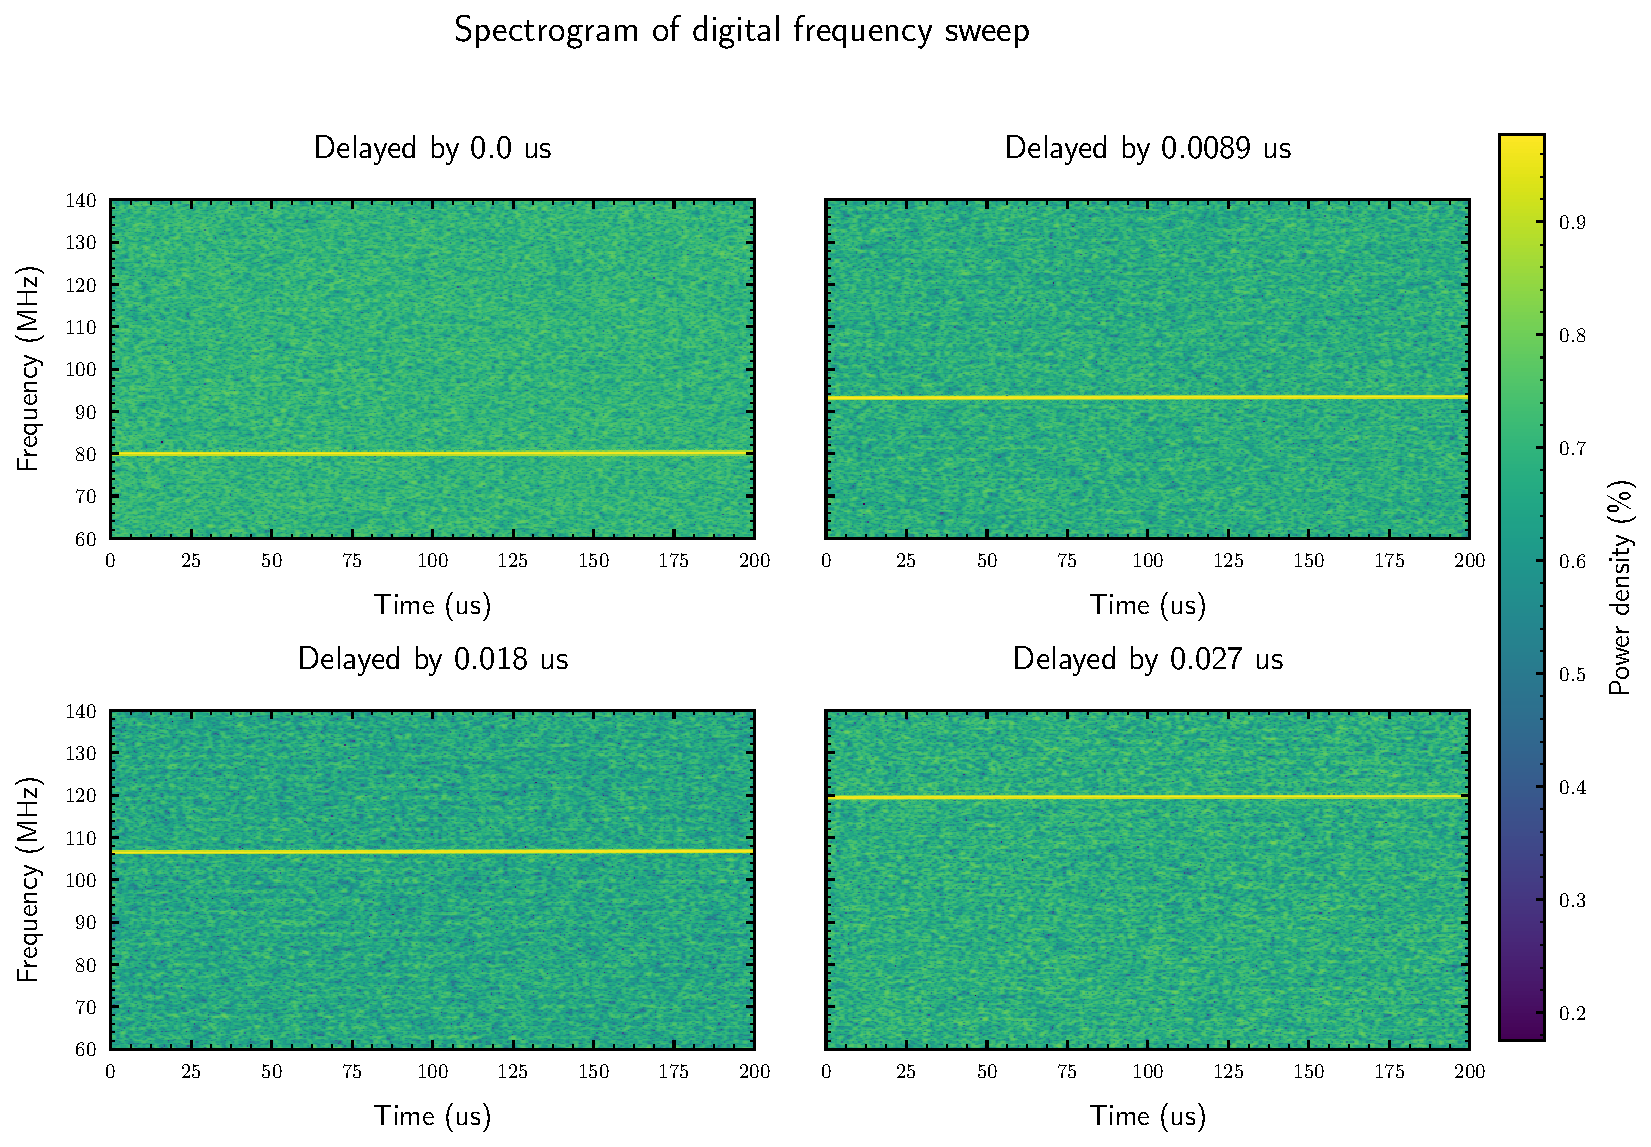
\includegraphics[width=\textwidth]{\figuredir{signal/synthesis/spectrogram.pdf}}
  \captionsetup{width=.8\textwidth}
  \caption{Spectrogram of delayed time windows of the \gls{dds} output signal
    configured to perform a linear frequency sweep. For an ideal linear sweep
    we would expect a linear timeline of the frequency, instead we observe a
    discrete set of frequencies.}
  \label{fig:signal_synthesis_spectrogram}
\end{figure}

\Cref{fig:signal_synthesis_spectrogram} depicts four spectrograms, each taken
at a different time window of the frequency sweep passthrough. The first
spectrogram captures the start of the frequency sweep. We can see how for the
first \SI{200}{\micro\second} the \gls{dds} outputs only the start frequency
of \SI{80}{\mega\hertz} which then is increased by increments to reach the
final frequency of \SI{120}{\mega\hertz} as can be seen in the lower right
spectrogram at the end of the frequency sweep.

\subsection{Amplitude frequency response}
\label{subsec:signal_synthesizer_amplitude_frequency_response}

Although the previous section satisfied our curiousity, it did only confirm
made presumptions. We will now move on with the examination of the amplitude
frequency response which by all means shows unexpected behaviour.

In the Fourier space we can locate the dominant frequency at the maximum of
the power spectrum. That in mind we can reduce the previous obtained time
window measurements to pairs of dominant frequency and maximum amplitude.
Under the assumption that the maximum amplitude lies closely in range of the
mean amplitude we find the amplitude frequency response spectrum.

\begin{figure}[h]
  \centering
  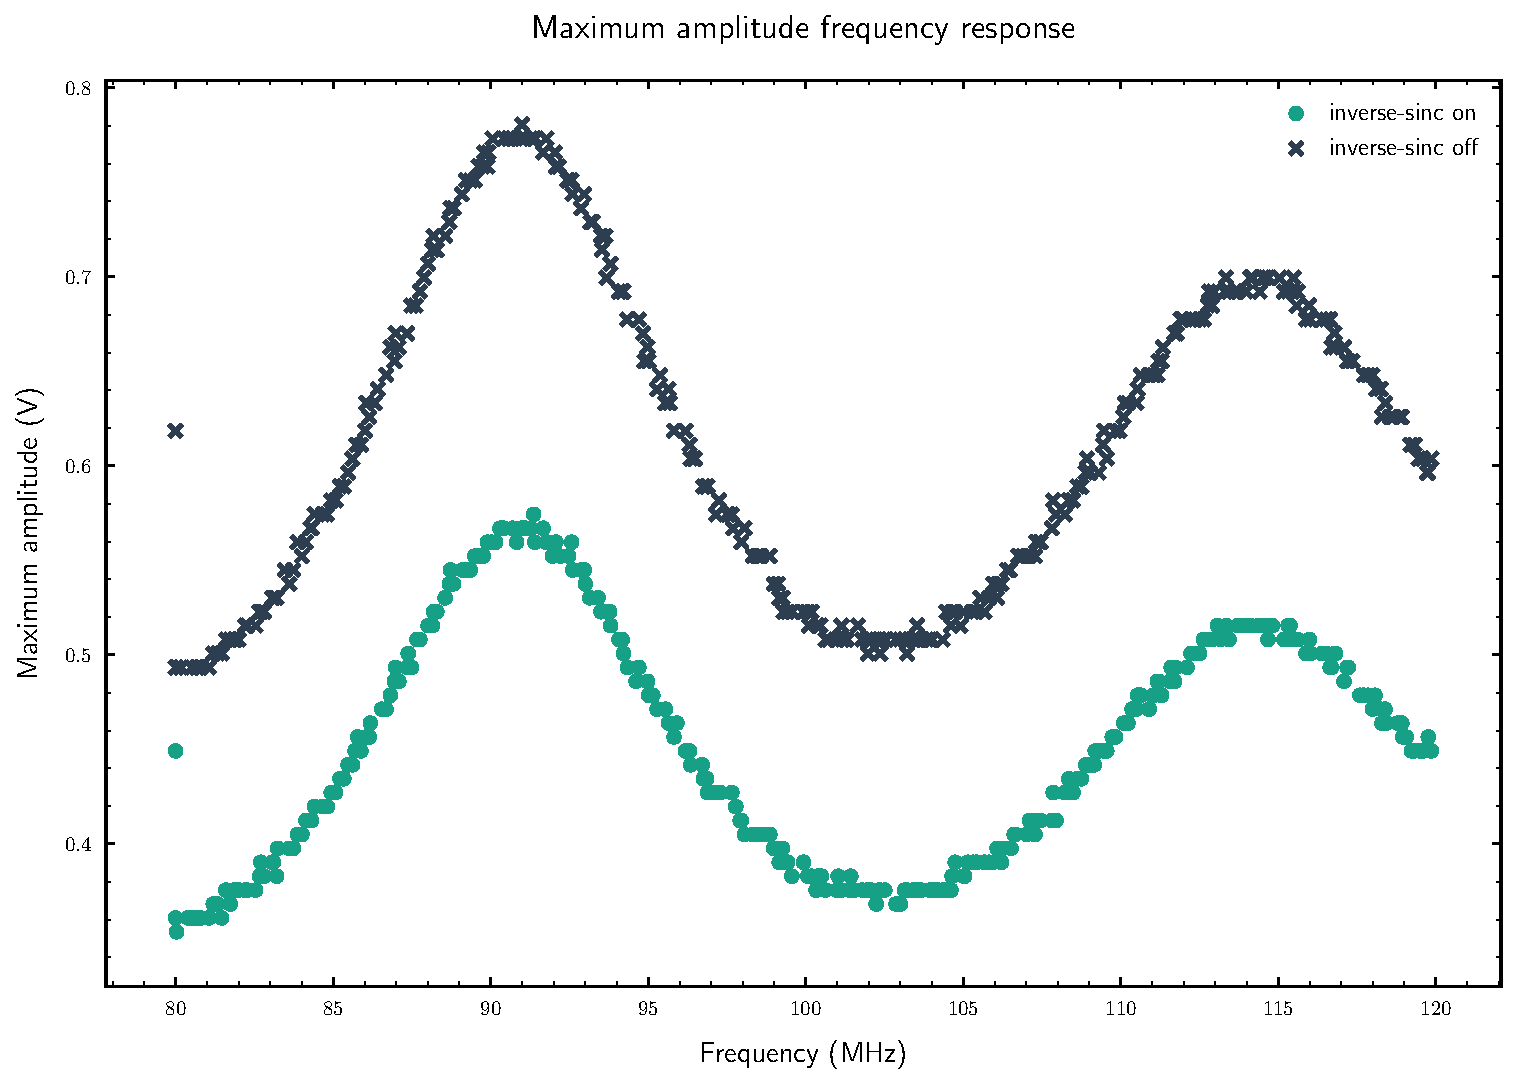
\includegraphics[width=.9\textwidth]{\figuredir{signal/synthesis/inverse-sinc.pdf}}
  \captionsetup{width=.9\textwidth}
  \caption{Maximum amplitude of the \gls{dds} signal output at different
    frequencies during linear sweep operation. In the bottom trace the
    \gls{dds} was configured with enabled inverse-sinc filter.}
  \label{fig:signal_synthesis_inverse_sinc}
\end{figure}

\Cref{fig:signal_synthesis_inverse_sinc} visualized the previously described
routine for the \gls{dds} assigned to the vertical \gls{aod}. The data
trace for the horizontal \gls{dds} is of equal shape, thus there are no
differences between the output signals of distinct \gls{dds} and we can limit
ourselves to the analysis of one such output. In
\Cref{fig:signal_synthesis_inverse_sinc} we can see a strong frequency
response of the amplitude. In particular we observe that at around
\SI{80}{\mega\hertz} and \SI{103}{\mega\hertz} the amplitude shows
significant local minima. The outliers on the left are caused by the no-dwell
mode enabled in the \gls{dds} configuration which causes the digital ramp to
return back to the start frequency and is necessary to support the external
trigger input. The datasheet of the \gls{ad9910} reports a characteristic
sinc dependency of the output power \cite{AD9910} and thus promotes a
built-in inverse-sinc filter to compensate in respect thereof. Having said
that the reported output power in dependency of the frequency in
\cite{AD9910} should only be of linear order for the investigated frequency
range and in fact as we can see in the lower trace in
\Cref{fig:signal_synthesis_inverse_sinc} the enabled inverse-sinc filter
does not account for our observed amplitude response.

\begin{figure}[h]
  \centering
  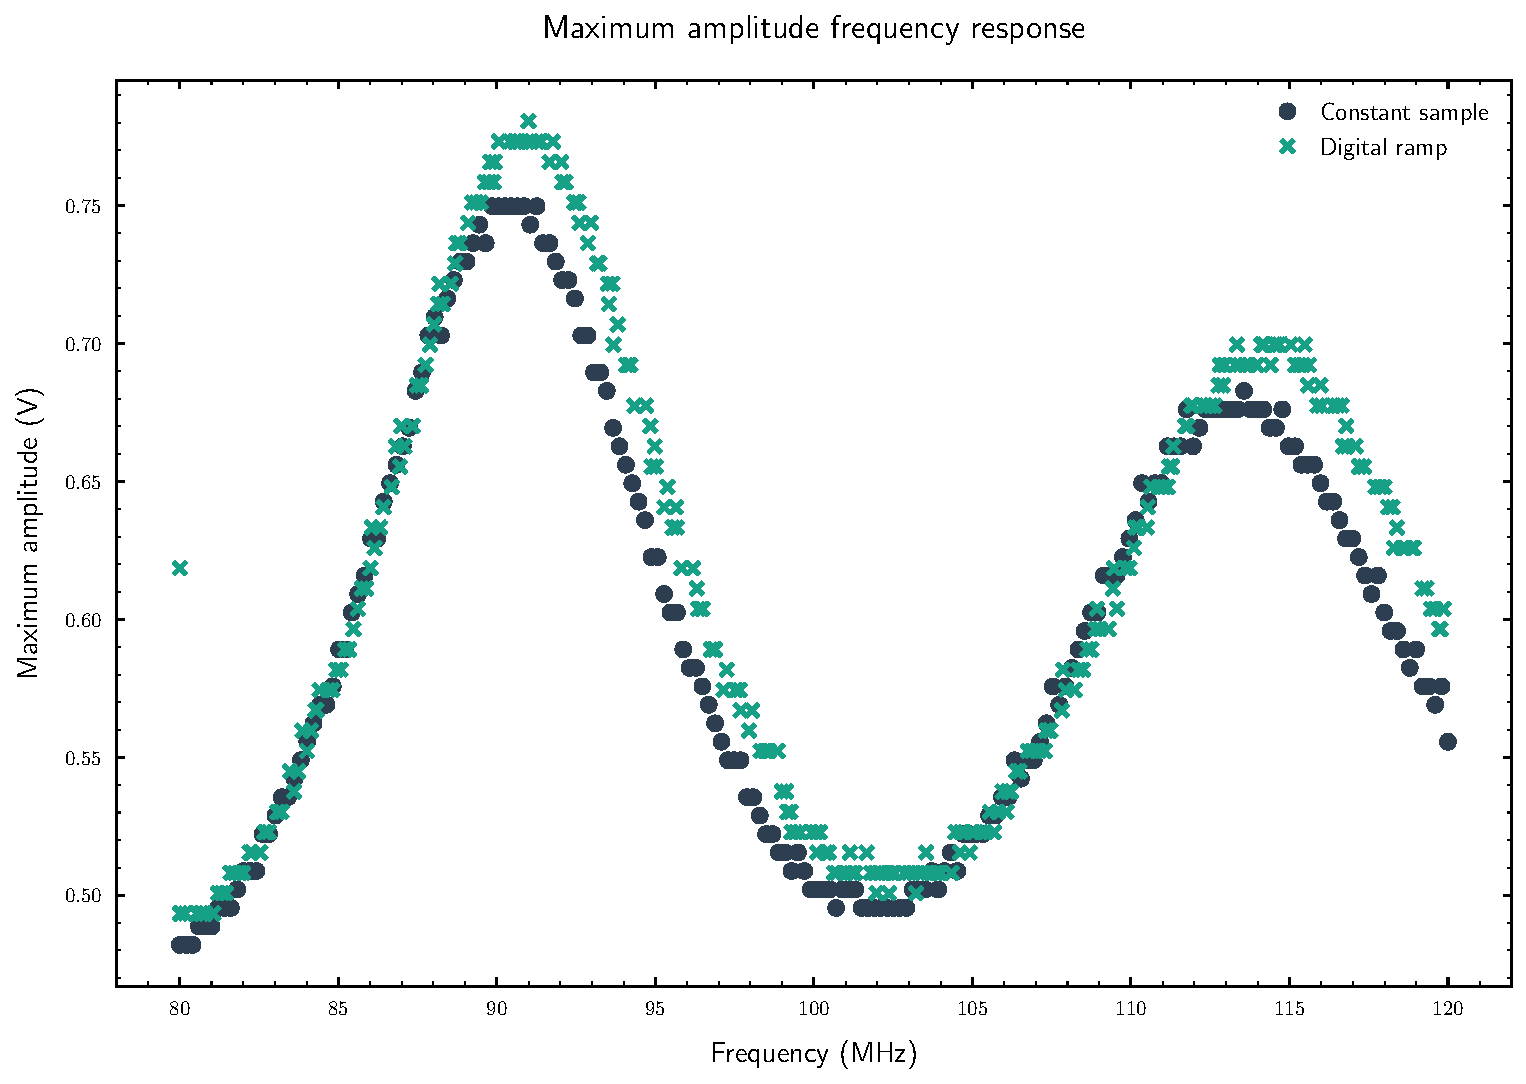
\includegraphics[width=.9\textwidth]{\figuredir{signal/synthesis/csample-dramp.pdf}}
  \captionsetup{width=.9\textwidth}
  \caption{Maximum amplitude of the \gls{dds} signal output at different
    frequencies once obtained by linear sweep operation and once through
    manual frequency sampling.}
  \label{fig:signal_synthesis_scample_dramp}
\end{figure}

One hypothesis suggested that the observed amplitude response is caused by
fact that the frequencies are sampled internally from the digital ramp logic.
Therefore we collected second data where we configured the vertical \gls{dds}
to output constant frequencies. The amplitude response for this setup is
disclosed in \Cref{fig:signal_synthesis_scample_dramp}. We can see that
indeed the digital ramp introduces a small frequency shift, nonetheless it
still shows the same global behaviour of the output power. Therefore we are
left unanswered with the origin of the observed output power spectrum.

\section{Power amplifier}

The piezoelectric attached to the acousto-optic crystal inside the \gls{aod}
elements has to emit acoustic waves strong enough to propagate through the
crystal structure of the acousto-optic crystal. Obviously such mechanical
method demands power not usually met by \gls{rf} signal sources such as the
\gls{dds}. Therefore it is essential to amplify the \gls{rf} signal through
a power amplifier.

\subsection{Amplitude frequency response}

The measurement procedure described in the previous section is still valid
for the now amplified signal of projected \SI{33}{\decibel\meter}. At the
usual \SI{50}{\ohm} in between coaxial cables this corresponds to an
approximate voltage of \SI{10}{\volt}. In order to protect the oscilloscope
for potential damage caused by too much power, we inserted a chain of
attentuators, from coaxial cable to oscilloscope \SI{1}{\decibel},
\SI{3}{\decibel}, \SI{6}{\decibel}, \SI{10}{\decibel} and \SI{10}{\decibel}
(to distribute heat dissipation) in between the coaxial cable and the
oscilloscope input to attain a total damping of \SI{30}{\decibel}. Otherwise
data analysis was performed analogue to the unamplified case.

\begin{figure}[h]
  \centering
  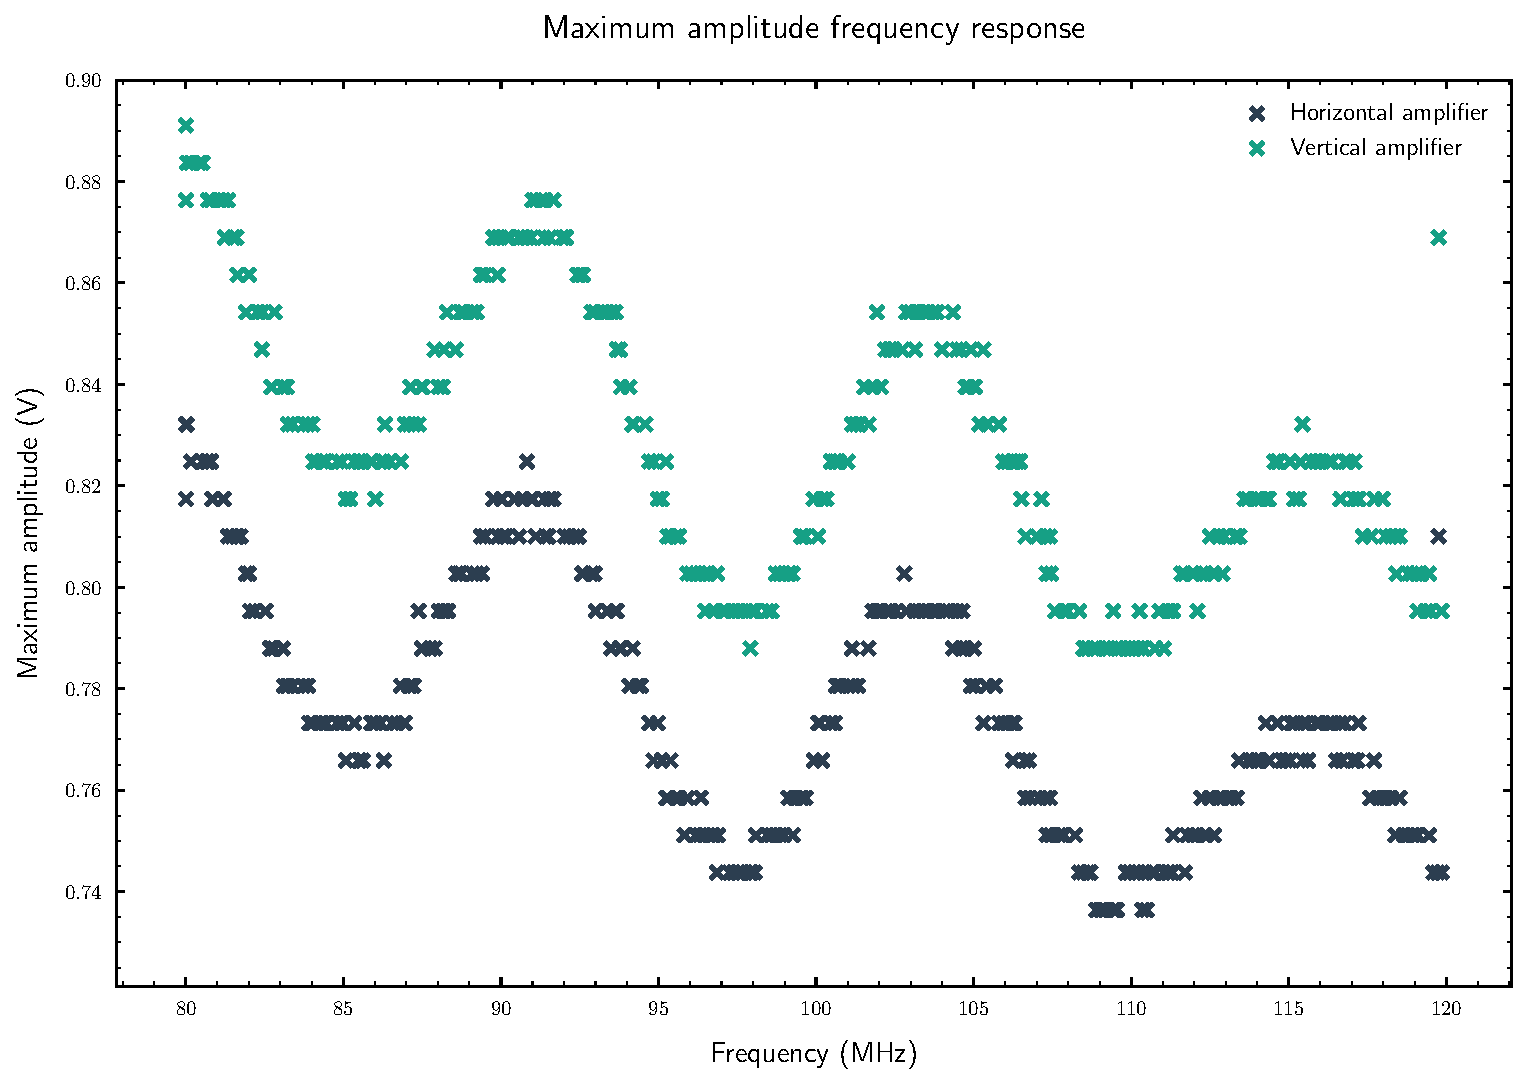
\includegraphics[width=.9\textwidth]{\figuredir{signal/amplification/amplitude-response.pdf}}
  \captionsetup{width=.9\textwidth}
  \caption{Maximum amplitude at dominant frequency per delayed window for two
  different amplifiers. We can see the discreteness of the frequency domain
from the digital signal synthesis as well as three resonances. Further the
amplifier differ by a constant offset.}
  \label{fig:signal_amplification_frequency_max_amplitude}
\end{figure}

\Cref{fig:signal_amplification_frequency_max_amplitude} presents us the
damped output signal subject to the signal frequency after amplification for
the two distinct amplifiers. We require two distinct amplifiers because our
setup comprises two independently controlled \gls{aod}.

At first we note that the amplified signal differs by a constant offset. We
assume this offset to be caused by different component quality as the
frequency response shape itself is similar. On a second glance we again find
evidence for discrete frequencies from
\Cref{fig:signal_amplification_frequency_max_amplitude} when we emphasize the
subtile horizontal pattern of the markers.

\begin{figure}[h]
  \centering
  \includegraphics[width=.9\textwidth]{\figuredir{signal/amplification/comparison.pdf}}
  \captionsetup{width=.9\textwidth}
  \caption{Relative amplitude at dominant frequency per delayed window for
  two different amplifiers and their digital signal source. In comparison to
the signal source the amplifiers introduce a further resonance at the
center frequency.}
  \label{fig:signal_amplification_comparison}
\end{figure}

\Cref{fig:signal_amplification_comparison} shows the min-max-normalized
amplified signals with the min-max-normalized input signal from the horizontal
\gls{dds}. After normalization the fixed offset difference, we observed
previously in between the distinct amplifiers, vanishes and the same
frequency response shape is obvious.

Comparison of the signal after (black, green) and before amplification (red)
yields that the input signal from \gls{dds} seems more dense than after the
amplification, yet we miss a solid explaination for this behaviour. It could
be that the selected voltage resolution of the oscilloscope was not optimal.
Furthermore we observe that the amplifier remedies the amplitude drop
at around \SI{102}{\mega\hertz} of the source signal. However the amplifier
possess resonances around \SI{98}{\mega\hertz} and \SI{110}{\mega\hertz}
where the amplitudes drop.

\subsection{Network analyzer transmission}

We previously discovered that the amplifier amends the frequency amplitude
response, nevertheless it is difficult to isolate the actual influence of
the amplifier and to preclude interaction effects caused by the already
unideal \gls{dds} signal. Therefore we conducted more detailed measurements
of the amplifiers power transmission with the network analyzer. The network
analyzer is a device that can measure reflection and transmission parameters
of electric components and does provide a cleaner input signal then used in
the previous measurement.

As in the measurement with the oscilloscope we also have to protect the
network analyzer against the output power of the amplifier. This time we
used a single \SI{30}{\decibel} attentuator in between the network analyzer
input and the power amplifier output.

\begin{figure}[h]
  \centering
  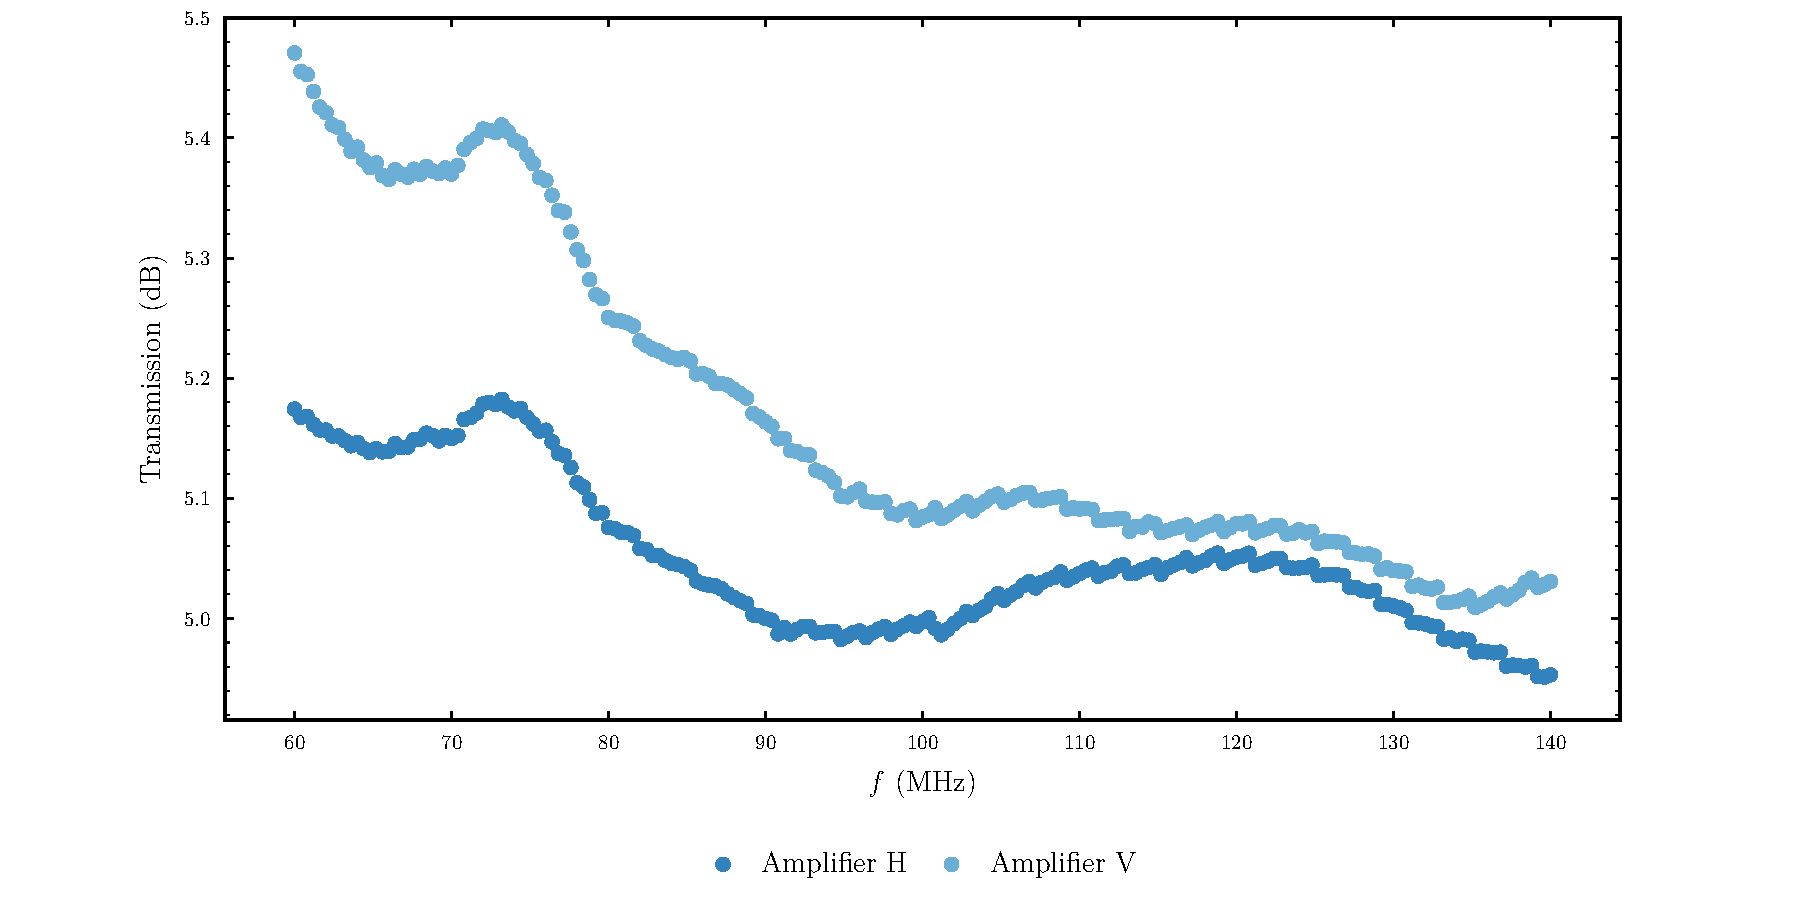
\includegraphics[width=.9\textwidth]{\figuredir{signal/amplification/transmission.pdf}}
  \captionsetup{width=.9\textwidth}
  \caption{Frequency transmission spectrum obtained via the network analyzer
  of the horziontal and vertical amplifiers.}
  \label{fig:signal_amplification_spectrum}
\end{figure}

In \Cref{fig:signal_amplification_spectrum} we see the frequency transmission
spectrum obtained through the network analyzer connected to the horizontal
and vertical amplifiers. We again can confirm a fixed offset of the
amplification gain between both amplifiers. Further we note that the
amplification factor falls of linearly in first order towards higher
frequencies.

\section{Acoustic transducer}

In the previous sections we explored the signal transfer at the synthesis
and amplification stage. The last stage that is accessable to us without
destruction of the \gls{aod} concerns the power reflection at the \gls{aod}
itself. From the reflection we can deduce the power transmission, hence for
a large reflection we would expect a small transmission and in that sense
less beam intensity in the first deflection order.

\subsection{Reflection spectrum}

The power reflection measurements were conducted with the network analyzer
we already introduced on the power amplifiers. In a first embodiment of the
experiment we directly supplied the \gls{aod} through a coaxial cable of the
network analyzer with power and measured the reflection. In a second
embodiment we used a direct-coupler to supply the respective amplifier with a
signal and measure the reflection through a direct-coupler.

\subsubsection{Direct connection}

\Cref{fig:signal_reflection_direct} visualizes the power reflection spectrum
of both \gls{aod} elements when directly connected to the network analyzer at
a maximum output power of \SI{10}{\decibel\meter}.

\begin{figure}[h]
  \centering
  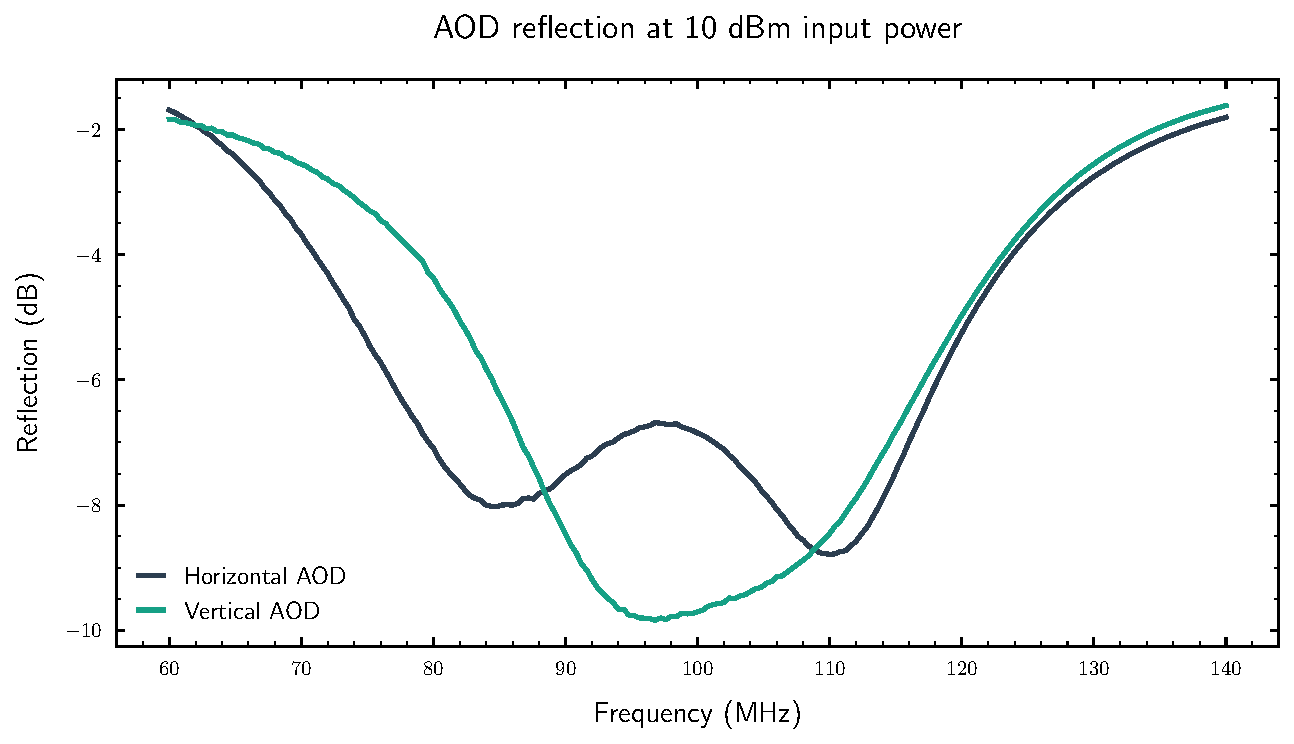
\includegraphics[width=.9\textwidth]{\figuredir{signal/reflection/direct.pdf}}
  \captionsetup{width=.8\textwidth}
  \caption{Signal reflection of the two different \gls{aod} when directly
    connected to the network analyzer.}
  \label{fig:signal_reflection_direct}
\end{figure}

The most interesting finding in \Cref{fig:signal_reflection_direct} is that
the power reflection shows very different behaviour in between the distinct
\gls{aod} elements. The \gls{aod} anticipated for the vertical deflection
is most transmissive at \SI{97}{\mega\hertz} with transmission falling of
on both sides while the \gls{aod} anticipated for the horizontal deflection
has two local transmission maxima and a rather bad transmision near the center
frequency.

\subsubsection{Amplified coupled connection}

In the second procedure we amplify the signal and couple the network analyzer
through a direct-coupler to measure the refleciton. This is done in order to
avoid harm to the network analyzer and because the network analyzer is not
able to provide \SI{2}{\watt} of output power as required by the \gls{aod}.

\begin{figure}[h]
  \centering
  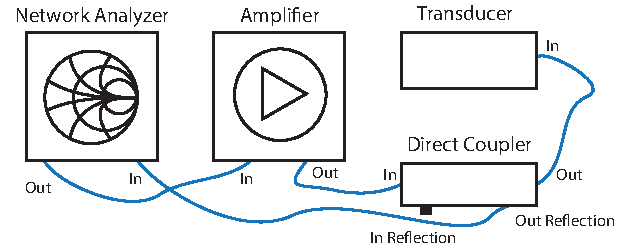
\includegraphics[width=.8\textwidth]{\mediadir{setup/transducer.pdf}}
  \captionsetup{width=\textwidth}
  \caption{Experimental setup to measure the reflection at the acouso-optic
  transducer component. The network analyzer supplies an input signal to
  the amplifier. The output signal of the amplifier is connected through
  a direct-coupler with the acousto-optic element. The direct-coupler allows
  to safely measure input and output reflection.}
  \label{fig:signal_amplification_transducer_setup}
\end{figure}

This setup is depicted in \Cref{fig:signal_amplification_transducer_setup}.
The network analyzer on the left-hand side supplies an input signal to the
amplifier. The input signal changes in linear in frequency. The output signal
of the amplifier is connected through a direct-coupler with the acousto-optic
element. The direct-coupler allows to safely measure input and output
reflection. 

The direct-coupler is an apparatus comprising a coaxial input and output
port as well as a coaxial input reflection and output reflection port. It is
disignated to measure the reflection of a (possible) high power signal
without jeopardizing measurement equipement.

\begin{figure}[h]
  \centering
  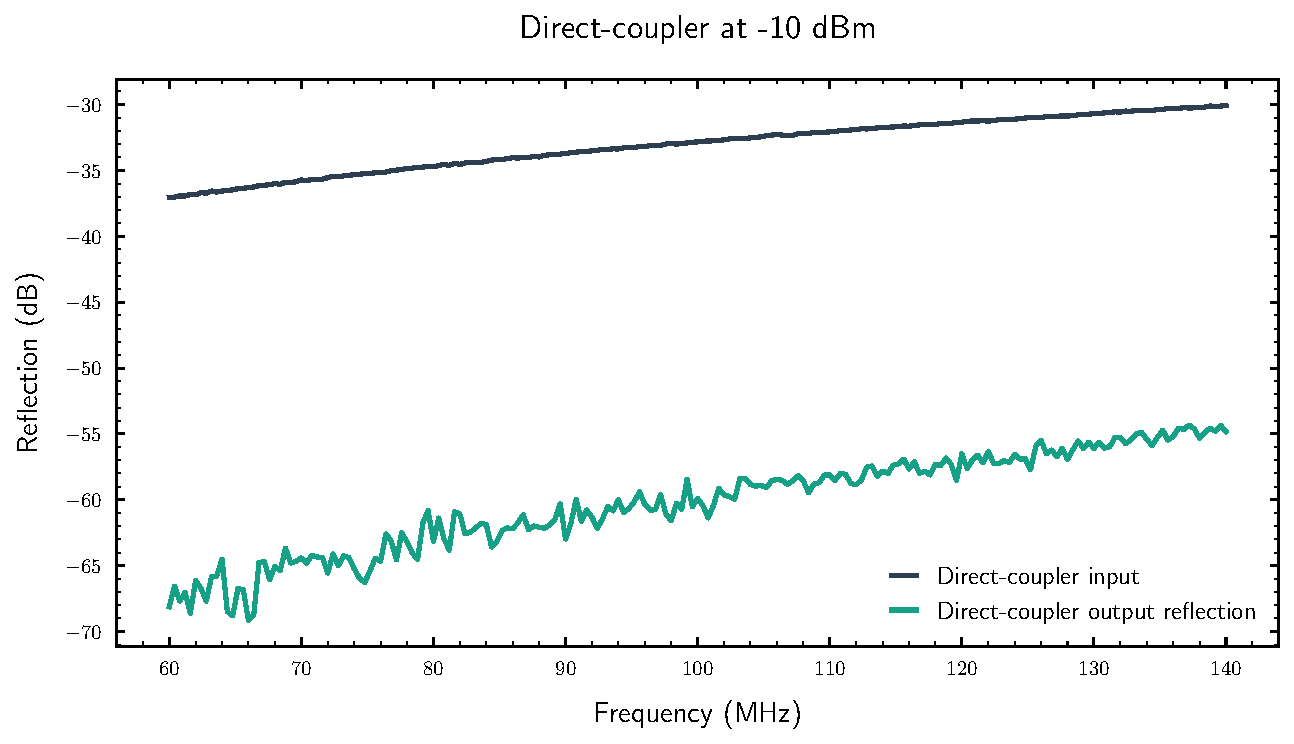
\includegraphics[width=\textwidth]{\figuredir{signal/reflection/coupler.pdf}}
  \captionsetup{width=.8\textwidth}
  \caption{Input power reflection when supplying the direct-coupler with
    \SI{-10}{\decibel\meter} input signal and reflection at the output of
    the direct-coupler while other ports are closed with \SI{50}{\ohm}}.
  \label{fig:signal_reflection_coupler}
\end{figure}

In \Cref{fig:signal_reflection_coupler} we see the reflection spectrum for
the case that we provide the network analyzer output signal to the input of
the direct-coupler and connect the reflection output of the direct-coupler
with the second network analyzer port while the remaining ports are under
\SI{50}{\ohm} closure.

We note that the reflection measured at through the direct-coupler is lowered
by many orders of magnitude compared to the input signal but essentially of
the same shape. The noise in the reflection is very high because of the low
power supplied into the direct-coupler.

We now use the direct-coupler to measure the output reflection at the
\gls{aod} elements after the signal was amplified.

\begin{figure}[h]
  \centering
  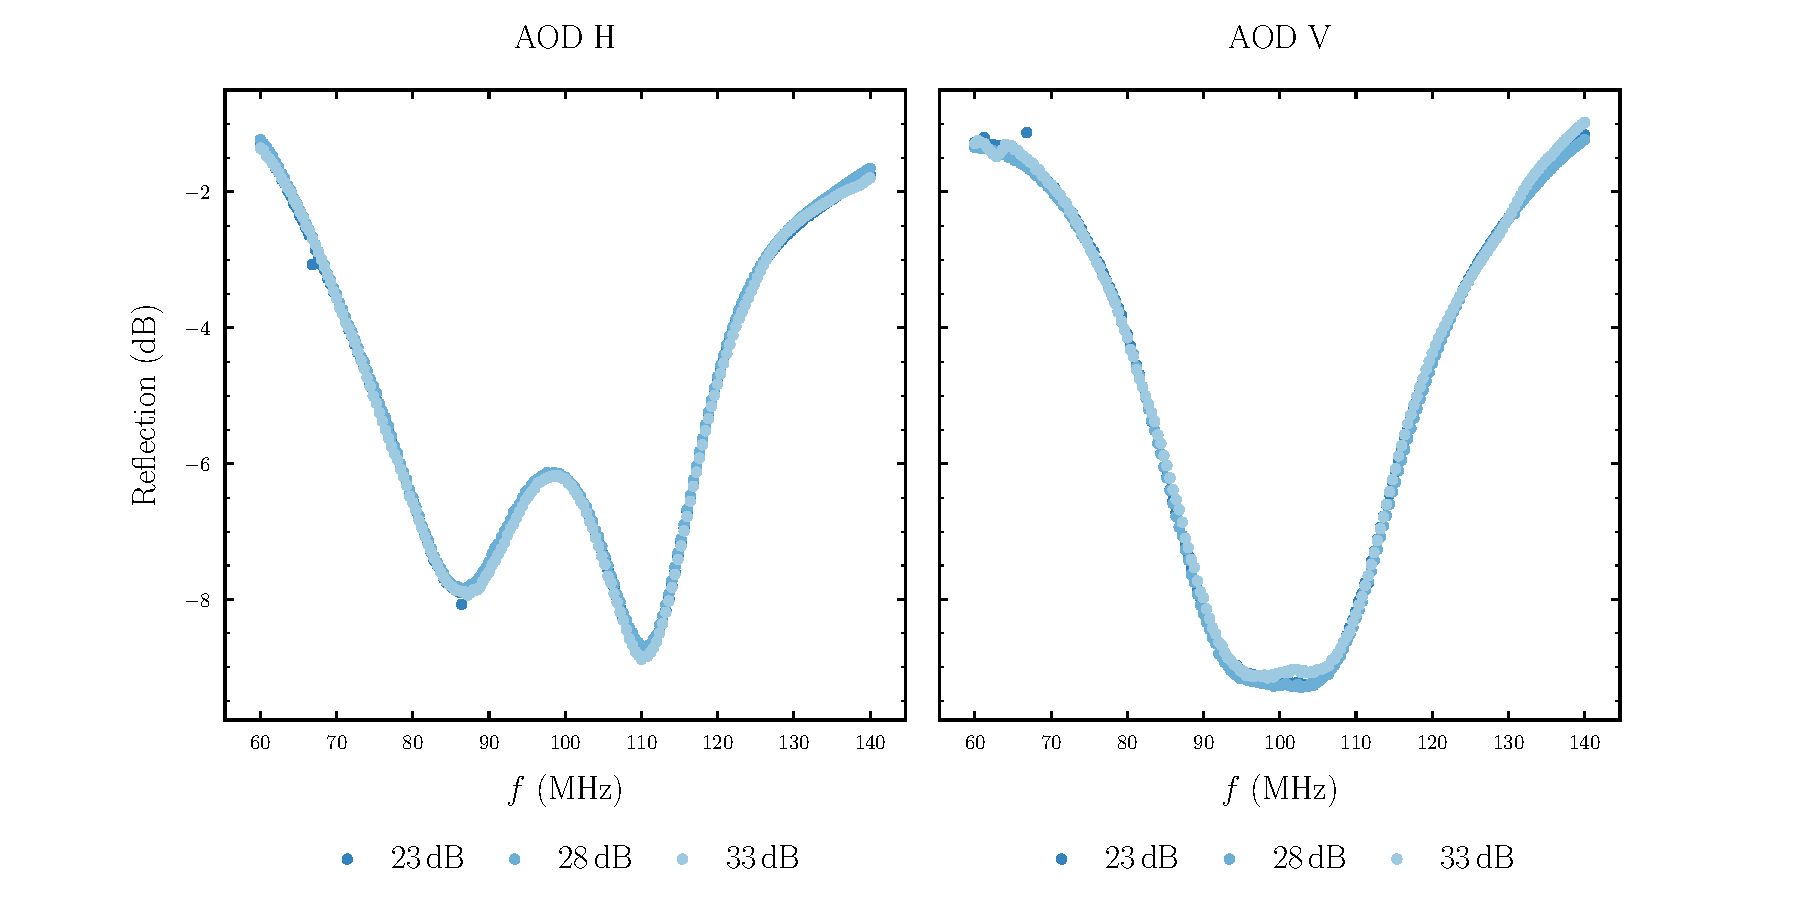
\includegraphics[width=\textwidth]{\figuredir{signal/reflection/coupled.pdf}}
  \captionsetup{width=.8\textwidth}
  \caption{Reflection at the direct-coupler output after amplification of the
  network analyzer input signal for different effective powers. We see that
the applied power does not effect the spectrum.}
  \label{fig:signal_reflection_coupled}
\end{figure}

In \Cref{fig:signal_reflection_coupled} we see the effective reflection
spectrum for the distinct \gls{aod} elements. The effective reflection
spectrum is obtained when subtracting the input reflection from the output
reflection.

\subsubsection{Comparison}

In the previous part we saw that the reflection spectrum does not show any
power dependence, thus we should be able to compare the spectrum we obtained
directly with the amplified result.

\begin{figure}[h]
  \centering
  \includegraphics[width=\textwidth]{\figuredir{signal/reflection/comparison.pdf}}
  \captionsetup{width=.8\textwidth}
  \caption{Comparison of reflection from amplified input signal and direct
  signal provided from the network analyzer. The different reflection spectrum
can be associated to the amplifier.}
  \label{fig:signal_reflection_comparison}
\end{figure}

In \Cref{fig:signal_reflection_comparison} we can see how there is additional
reflection from the amplifier, nevertheless the global spectrum
characteristics stay in place.

\subsubsection{Summary}

Distinct \gls{aod} elements show different power transmission characteristics
independent of the applied power. Examination of the \gls{aod} elements in
details discloses different impedance matching circuits.

Impedance matching is used to reduce power reflection by providing a constant
input resistance of \SI{50}{\ohm} accross an ideally wide frequency range.
Still the impedance differs between the \gls{aod}s. We assume that the
crystal properties i.e. cut, purity are responsible for that.

By the previous reflections measurements we keep in mind that these were
conducted with an input signal with fairly homogenous amplitude. From the
previous sections we know that this in fact is not the case for the \gls{rf}
signal later used.
